\section{Results}\label{sec:results}
    To validate this new feature, we performed a parameter scan study on a PWR
    pincell using a single depletion zone. Tables \ref{tab:mat-params},
    \ref{tab:fuel-comp}, \ref{tab:clad-comp}, and \ref{tab:water-comp} contain
    the material parameters of our model, and Table \ref{tab:geo-params}
    contains the geometric parameters.  We used the ENDF/B-VII.1 nuclear data
    library available at \url{openmc.org/official-data-libraries}. We used the
    ENDF/B-VII.1 depletion chain in the PWR spectrum available at
    \url{openmc.org/depletion-chains}.
    
    \begin{table}[<options>]
        \caption{Material Parameters}
        \label{tab:mat-params}
        \begin{tabular*}{\tblwidth}{@{}LLLL@{}}
            \toprule
             Item & Fuel & Cladding & Water \\ % Table header row
            \midrule
             Density [g cm$^{-3}$] & 10.4 & 6 & 1.0\\
             Volume [cm$^{3}$] & 0.1764$\pi$ & -- & -- \\
             S($\alpha$,$\beta$) & --  & -- & \verb.c_H_in_H2O.\\
            \bottomrule
        \end{tabular*}
    \end{table}

    \begin{table}[<options>]
        \caption{Fuel Composition}
        \label{tab:fuel-comp}
        \begin{tabular*}{\tblwidth}{@{}LL@{}}
            \toprule
            Nuclide & Composition [atom \%] \\ % Table header row
            \midrule
             $^{15}$O & 0.000758 \\
             $^{16}$O & 1.999242 \\
             $^{234}$U & 0.000385 \\
             $^{235}$U & 0.043020 \\
             $^{236}$U & 0.000197 \\ 
             $^{238}$U & 0.956398 \\
             \bottomrule
        \end{tabular*}
    \end{table}

    \begin{table}[<options>]
        \caption{Cladding Composition}
        \label{tab:clad-comp}
        \begin{tabular*}{\tblwidth}{@{}LL@{}}
            \toprule
            Nuclide & Composition [atom \%] \\ % Table header row
            \midrule
             $^{90}$Zr & 0.5145 \\
             $^{91}$Zr & 0.1122 \\
             $^{92}$Zr & 0.1715 \\
             $^{94}$Zr & 0.1738 \\
             $^{96}$Zr & 0.028 \\ 
             \bottomrule
        \end{tabular*}
    \end{table}

    \begin{table}[<options>]
        \caption{Water Composition}
        \label{tab:water-comp}
        \begin{tabular*}{\tblwidth}{@{}LL@{}}
            \toprule
            Nuclide & Composition [atom \%] \\ % Table header row
            \midrule
             $^{1}$H & 1.999689\\
             $^{2}$H & 0.000311 \\
             $^{15}$O & 0.999621 \\
             $^{16}$O & 0.000379 \\
             \bottomrule
        \end{tabular*}
    \end{table}

    \begin{table}[<options>]
        \caption{Geometric Parameters}\label{tab:geo-params}
        \begin{tabular*}{\tblwidth}{@{}LLLL@{}}
            \toprule
            Fuel Radius [cm] & Clad Radius [cm] & Water Bounding Box dimensions
            [cm  $\times$ cm]\\
            \midrule
            0.42 & 0.45 &  1.24 $\times$ 1.24\\
            \bottomrule
        \end{tabular*}
    \end{table}
    We used time step size as our parameter to vary.
    Table \ref{tab:timestep-shorthands} shows the different time step sizes we
    used and their shorthand terminology. All simulations ran for 10 depletion
    steps.
    \begin{table}[<options>]
        \caption{}\label{tab:timestep-shorthands}
        \begin{tabular*}{\tblwidth}{@{}LL@{}}
            \toprule
            Time step sizes & Shorthand term \\ % Table header row
            \midrule
            360 seconds & Minutes\\
            4 hours & Hours\\
            3 days & Days\\
            30 days & Months\\
            \bottomrule
        \end{tabular*}
    \end{table}
    We used the \verb.PredictorIntegrator. time stepper, which is analagous to
    the Euler method. Predictor-corrector methods are not useful for transport
    independent depetion. The correction step will utilize the same reaction
    rates as the initial prediction due to the static fluxes and cross sections.
    This means any predictor-corrector method will produce the same numerical
    results as a predictor method but with higher floating-point errors due to
    the increased number of operations \footnote{Preliminary testing with
    predictor-corrector methods confirmed the highter floating point errors,
    however they are marginal in magnitude}.

    We used constant reacton rate Q values multiplied by the reaction rates to
    obtain the normalization factor $f$ (\verb.fission-q. normalization) for all
    cases with a linear power density of 174 W/cm. For each timestep size.
    we ran with three cases:
    \begin{enumerate}
        \item Transport-coupled depletion
        \item Transport-independent depletion
        \item Transport-independent depletion with microscopic cross sections
            updated after each depletion step (one-group only).
    \end{enumerate}

    For the first case, we used 25 inactive and 125 active batches, with $10^6$
    particles per batch. For transport independent depletion, we used three
    different group strucutres to test the effect on the accuracy: one group,
    CASMO-8, and CASMO-40.

    Note that the third case is significantly slower than transport-coupled
    depletion as the cross sections need to be reloaded after each depletion
    step. Due to the cross section discretization that occurs before peforming
    depletion, we do not expect the third case results to converge to the first
    case results in limit of infinite particles. We would expect the third case
    to converge in the limit of infinite particles and energy groups. The third
    case was only run for one-group transport-independent depletion. Unless
    otherwise specified, all results are using 3-day time steps and
    \verb.PredictorIntegrator. The general trend is that concentration errors
    are smaller for shorter depletion time steps, and larger for longer
    depletion time steps, however there are more complicated dynamics for this
    to be a reliable prediction for each nuclide concentration.

    % actinides error 
    \begin{figure}[h!tpb]
        \centering
        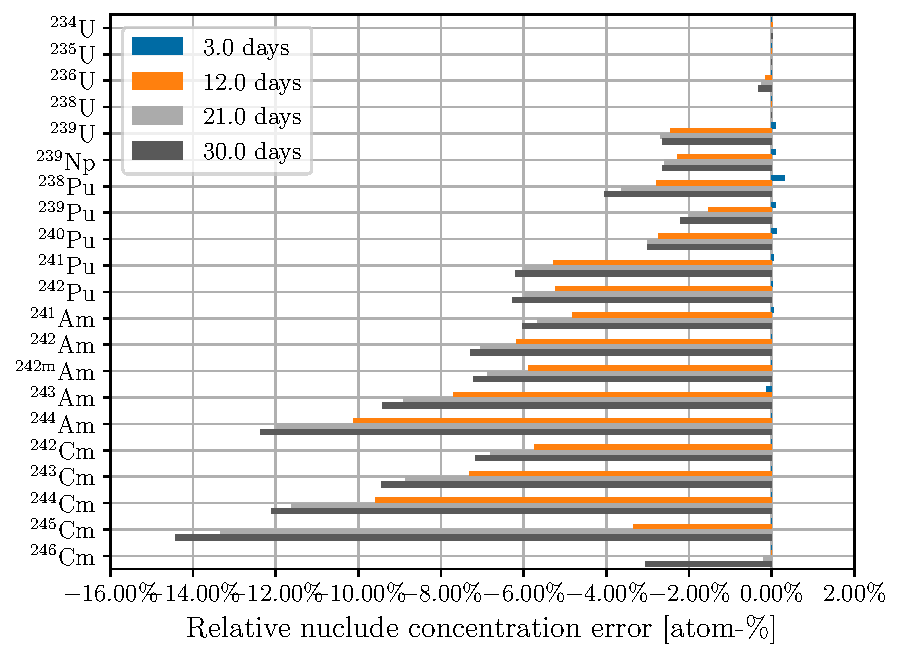
\includegraphics[width=\linewidth]{figs/actinides_constant_xs_predictor_fission_q_days.pdf}
        \caption[]{Relative error of predicted actinide concentrations using
        constant cross sections and 3-day time steps}
        \label{fig:actinides-error-constant-xs-days}
    \end{figure}

    \begin{figure}[h!tpb]
        \centering
        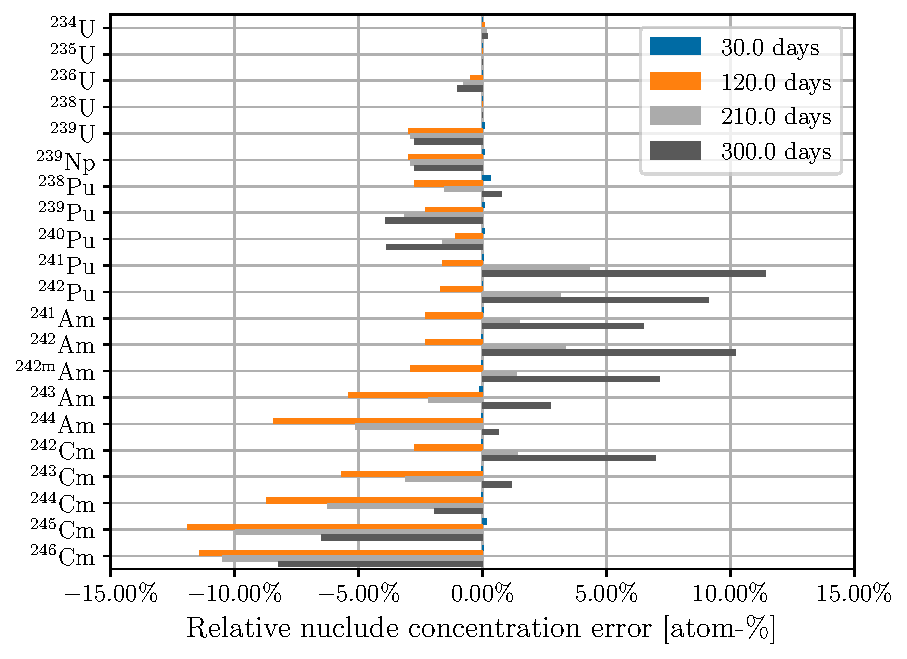
\includegraphics[width=\linewidth]{figs/actinides_constant_xs_predictor_fission_q_months.pdf}
        \caption{Relative error of predicted actinide error using
        constant cross sections and 30-day time steps}
        \label{fig:actinides-error-constant-xs-months}
    \end{figure}

    Figures \ref{fig:actinides-error-constant-xs-days} and
    \ref{fig:actinides-error-updating-xs-days} show the relative error for
    actinides using constant cross sections and updating cross sections,
    respectively, using 3-day time steps. Figures
    \ref{fig:actinides-error-constant-xs-months} and
    \ref{fig:actinides-error-updating-xs-months} show the same respective
    quantities for 30-day time steps. As expected, updating the cross sections
    at each depletion step results in very low errors, on the order of a
    fraction of a percent. The error trend for constant cross sections depends
    both on the cross section and time step size. For example, constant cross
    sections using a 3-day time step underpredicts the \ce{^{241}Pu}
    concentration, but at longer time steps overpredicts the concentration. The
    overprediction is due due to overcalculating the rate of ($n,\gamma$)
    reactions that occur on \ce{^{240}Pu}. Figure \ref{fig:pu240-n-gamma-months}
    shows this.

    \begin{figure}[htpb]
        \centering
        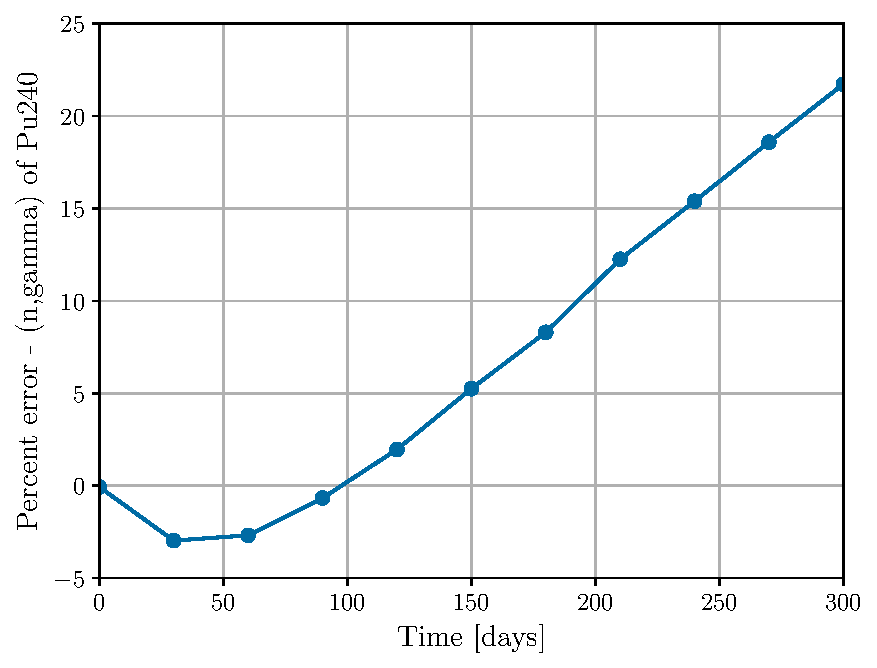
\includegraphics[width=\linewidth]{figs/pu240-n-gamma-months.pdf}
        \caption{Relative error of predicted \ce{^{240}Pu} ($n,\gamma$)
            reactions using constant cross sections and 30-day time steps}
        \label{fig:pu240-n-gamma-months}
    \end{figure}

    The error timeseries of \ce{^{241}Pu} is reproduced in daughter nuclides
    that are related to the amount of \ce{^{241}Pu}, such as isotopes of \ce{Cm}
    and \ce{Am}. We observe a general trend that the less important or abundant
    nuclides have higher concentration error relative to transport-coupled
    depletion. The less abundant actinides have increased sensitivity to over or
    underestimations of production.  The more important nuclides (\ce{U},
    \ce{^{239}Np}, \ce{^{239}Pu}, \ce{^{240}Pu}) tend to have low concentration
    errors, (5\% or less), whereas the less important actinides (Am, Cm,
    \ce{^{241}Pu}, \ce{^{242}Pu}) tend to have very high (more than 10\%)
    depending on the nuclide of interest.

    \begin{figure}[htpb]
        \centering
        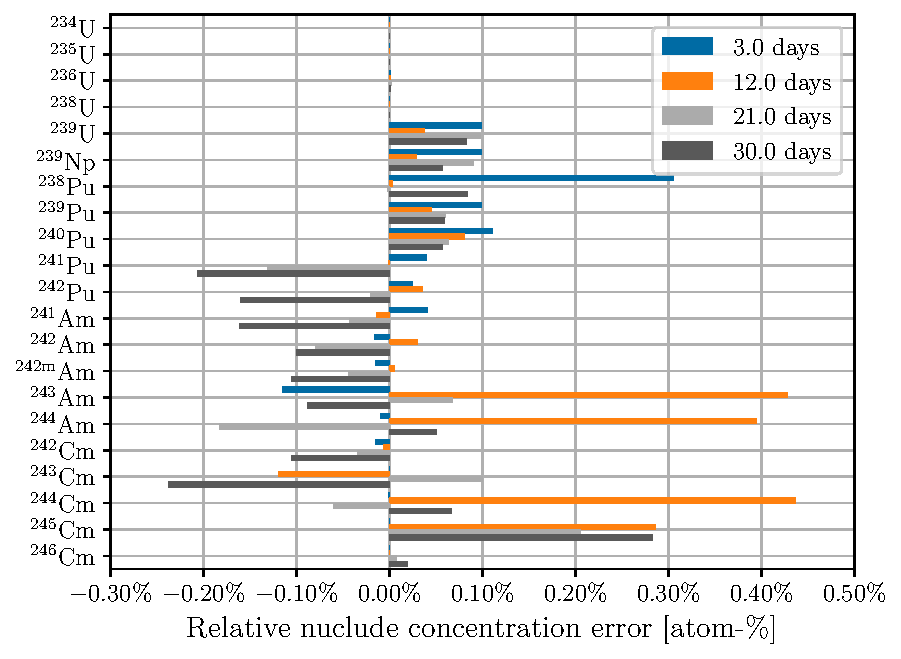
\includegraphics[width=\linewidth]{figs/actinides_updating_xs_predictor_fission_q_days.pdf}
        \caption{Relative error of predicted actinide error using
        updating cross sections and 3-day time steps}
        \label{fig:actinides-error-updating-xs-days}
    \end{figure}

    \begin{figure}[htpb]
        \centering
        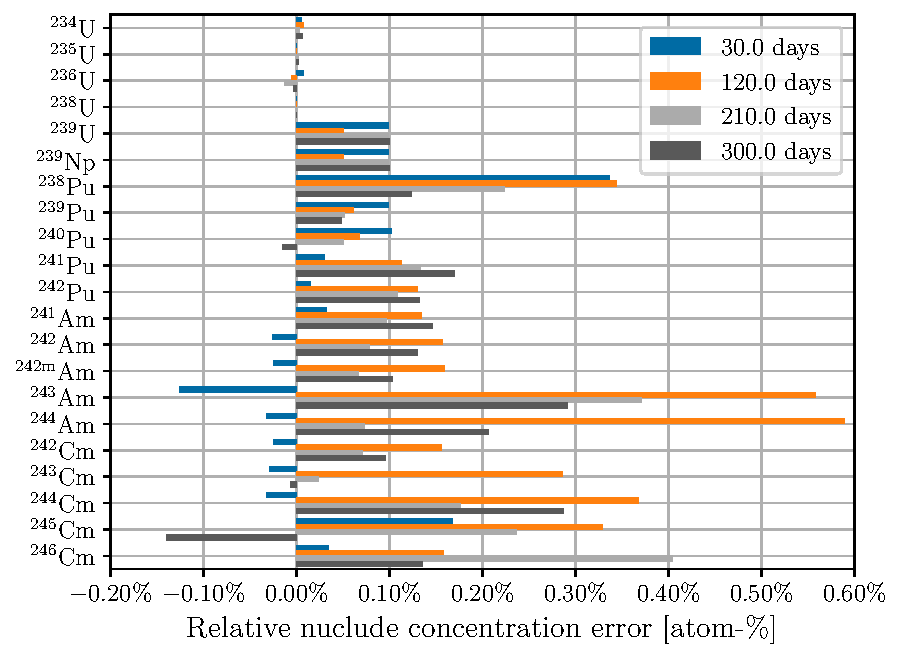
\includegraphics[width=\linewidth]{figs/actinides_updating_xs_predictor_fission_q_months.pdf}
        \caption{Relative error of predicted actinide error using
        updating cross sections and 30-day time steps}
        \label{fig:actinides-error-updating-xs-months}
    \end{figure}


    Figures \ref{fig:fp-error-constant-xs-days} and
    \ref{fig:fp-error-updating-xs-days} show the relative error for fission
    products using constant cross sections and updating cross sections,
    respectively, using 3-day time steps. Figures
    \ref{fig:fp-error-constant-xs-months} and
    \ref{fig:fp-error-updating-xs-months} show the same respective quantities
    for 30-day time steps. Similar to the actinides, updating the cross sections
    at each time step results in very low nuclide composition errors. There is a
    notably lower error across the board for many of these fission products
    compared to the actinides. This can simply be explained by the low
    composition error of \ce{^{235}U}. The majority of the fissile material in
    the fuel is \ce{^{235}U}, so the composition error of fission products
    produced should also be relatively low. Other actinides with higher
    composition errors are orders of magnitude less abundant in the fuel, so
    their effect on fission product composition error is proportionaly small.

    Composition errors for low-abundance nuclides using 30-day timesteps follow
    an interesting trend where there is an initial large negative error
    composition error that becomes more positive over time. This behavior is due
    to overestimation of nuclide production due to static cross sections and
    fluxes.

% fission products error
    \begin{figure}[h!tpb]
        \centering
        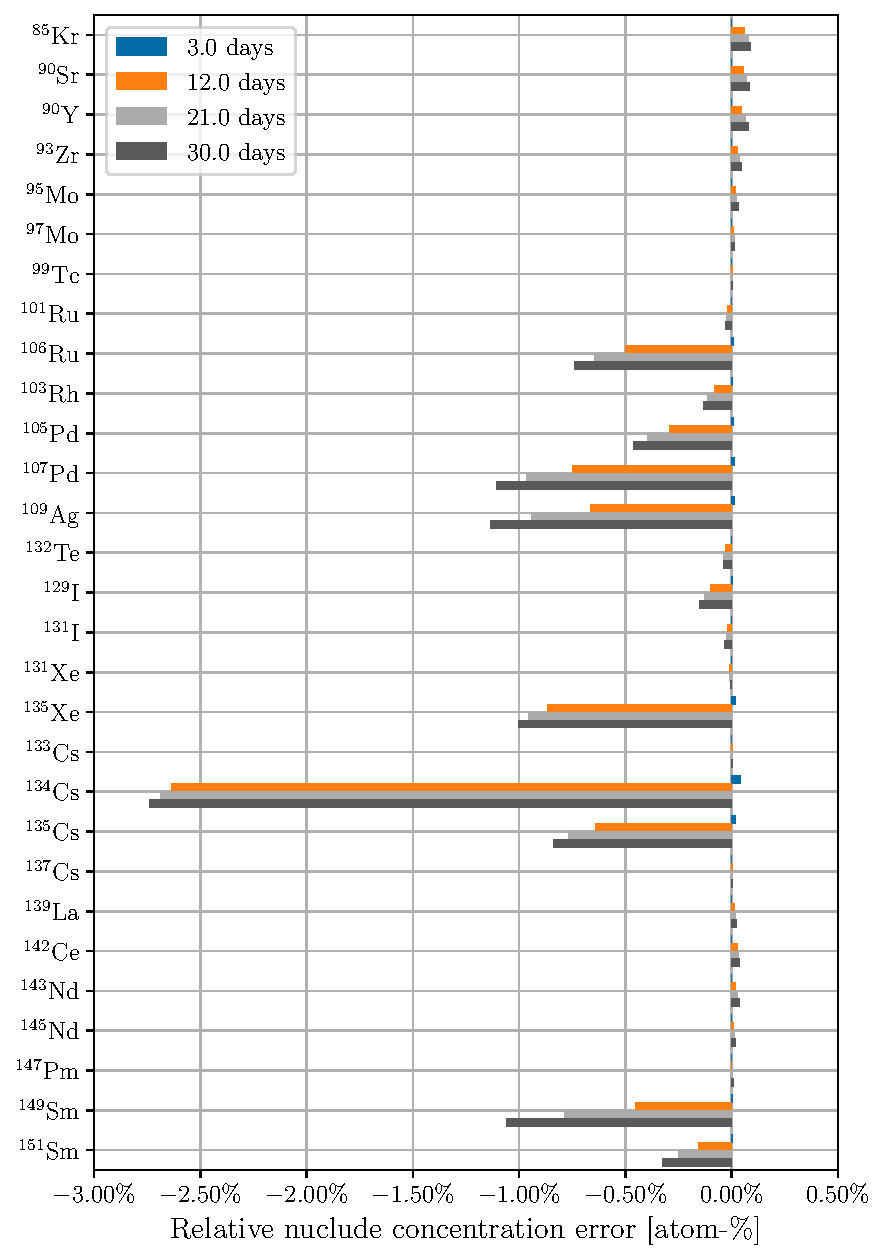
\includegraphics[width=\linewidth]{figs/fission_products_constant_xs_predictor_fission_q_days.pdf}
        \caption{Relative error of predicted fission product concentrations
        using constant cross sections and 3-day time steps}
        \label{fig:fp-error-constant-xs-days}
    \end{figure}

    \begin{figure}[htpb]
        \centering
        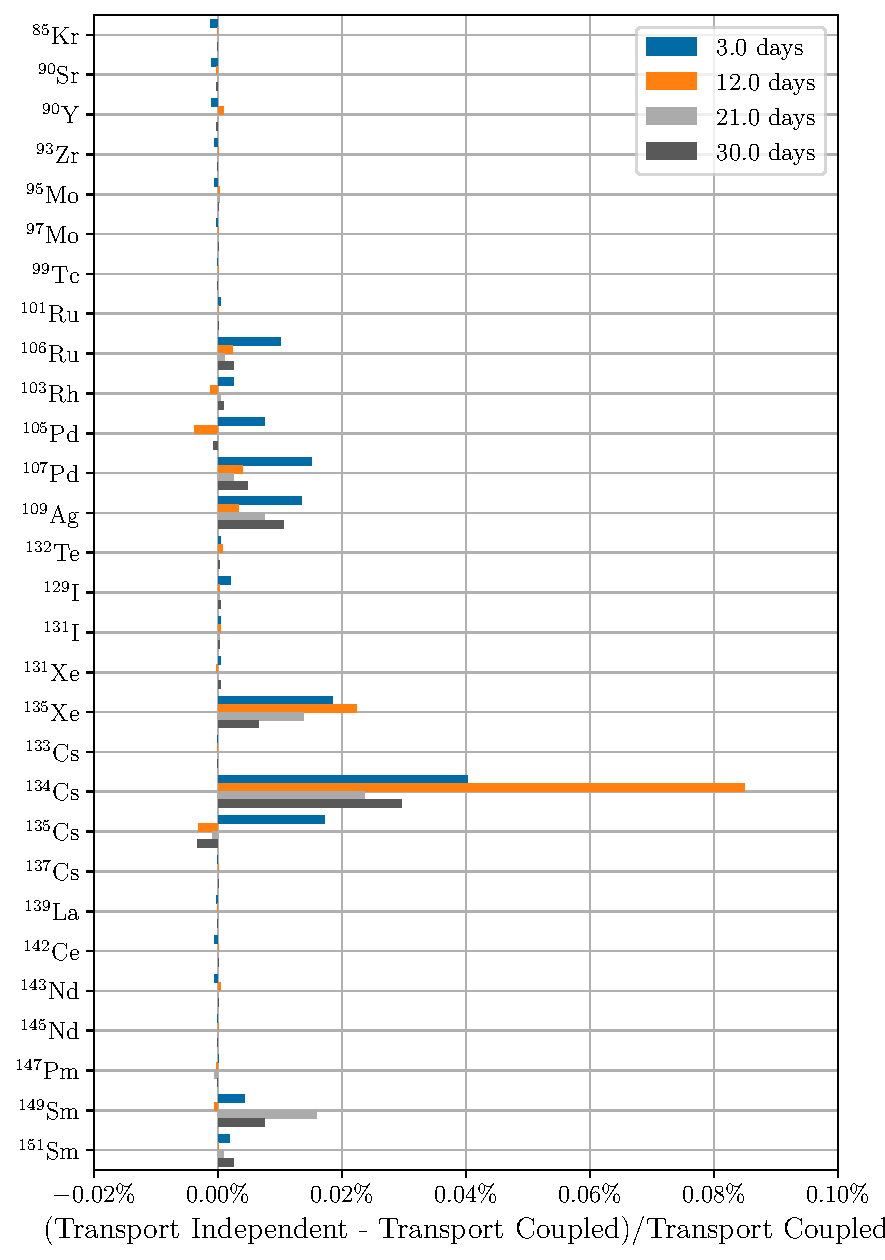
\includegraphics[width=\linewidth]{figs/fission_products_updating_xs_predictor_fission_q_days.pdf}
        \caption{Relative error of predicted fission product error using
        updating cross sections and 3-day timesteps}
        \label{fig:fp-error-updating-xs-days}
    \end{figure}
 
    \begin{figure}[htpb]
        \centering
        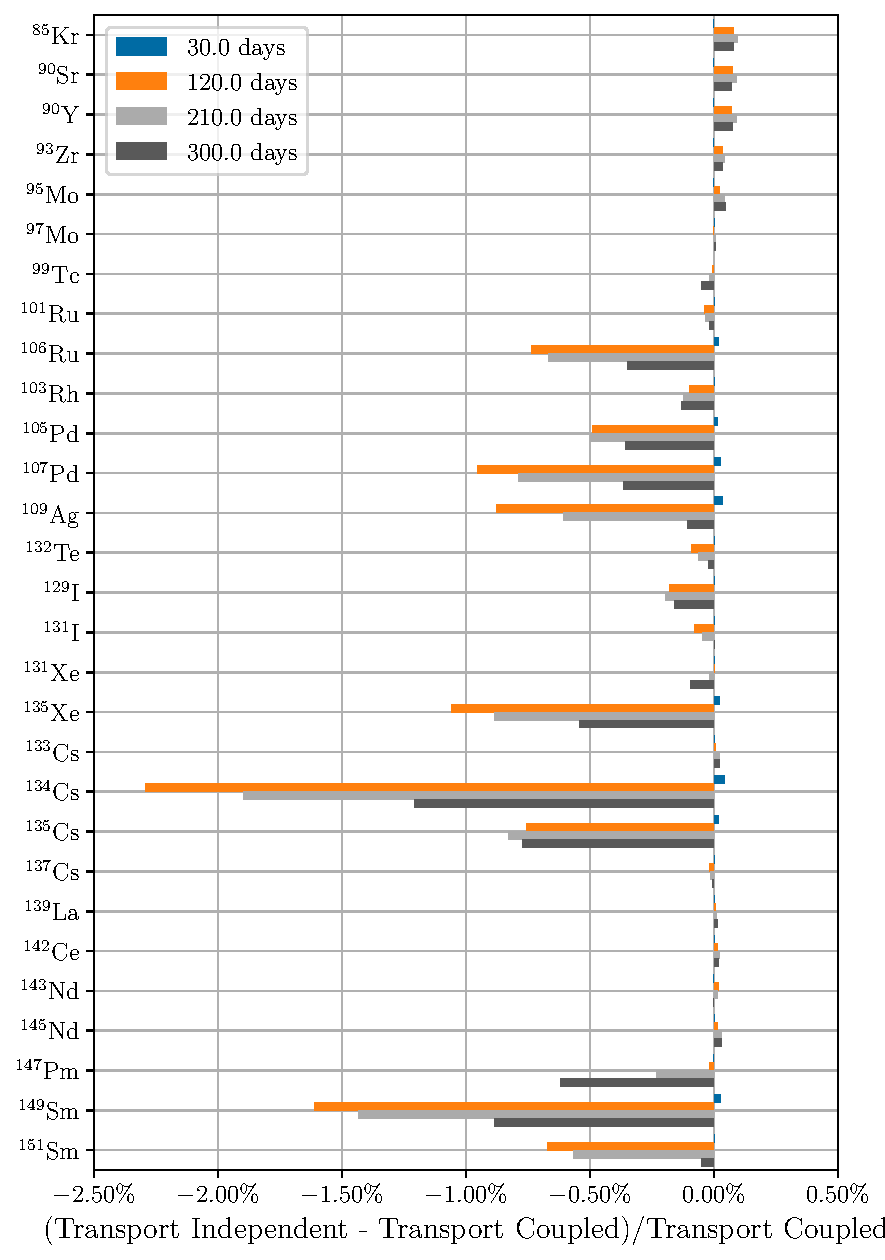
\includegraphics[width=\linewidth]{figs/fission_products_constant_xs_predictor_fission_q_months.pdf}
        \caption{Relative error of predicted fission product error using
        constant cross sections and 30-day time steps}
        \label{fig:fp-error-constant-xs-months}
    \end{figure}

    \begin{figure}[htpb]
        \centering
        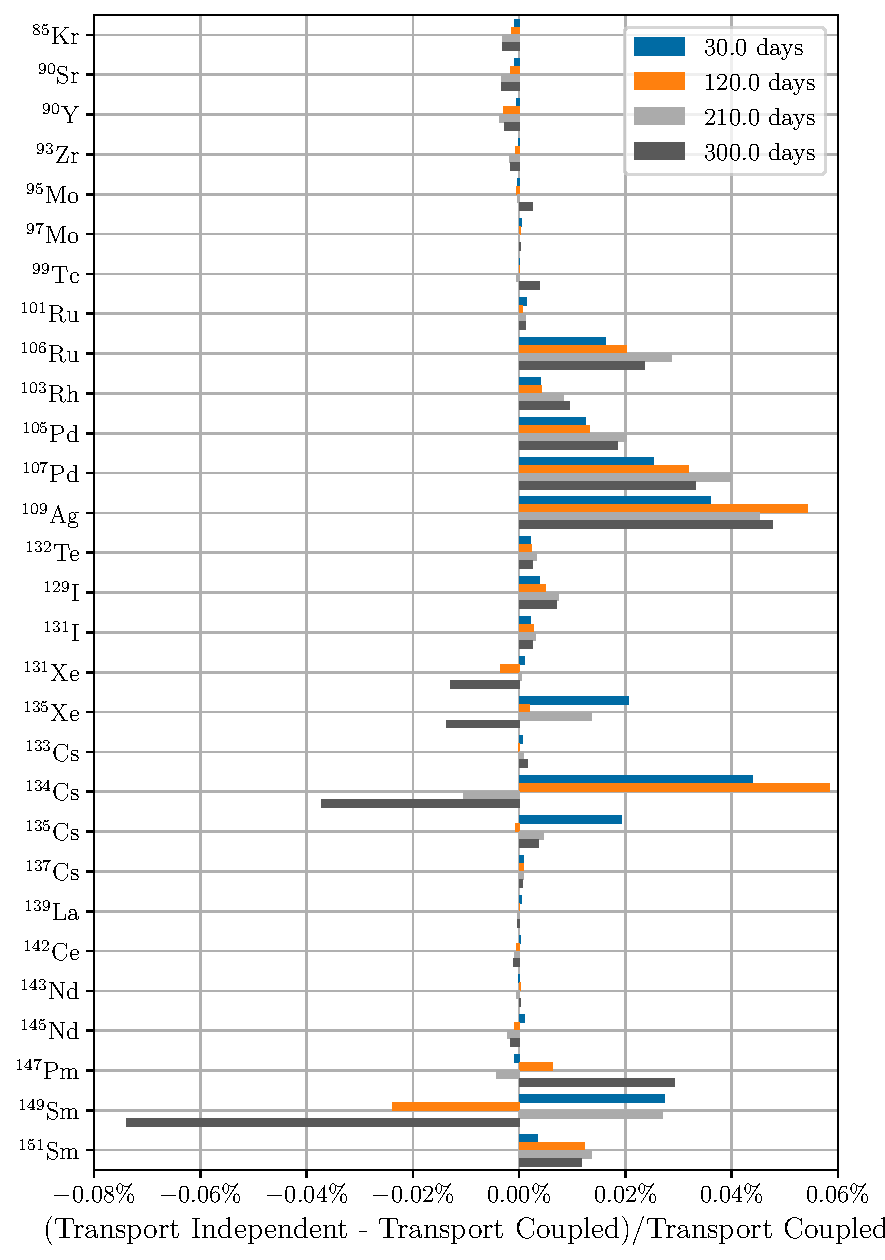
\includegraphics[width=\linewidth]{figs/fission_products_updating_xs_predictor_fission_q_months.pdf}
        \caption{Relative error of predicted fission product error using
        updating cross sections and 30-day time steps}
        \label{fig:fp-error-updating-xs-months}
    \end{figure}

    Repeating this analysis for both the CASMO-8 and CASMO-40 multi-group
    strucutres did not yield significant decreases in error for
    transport-independent depletion over the one-group case.  Figures
    \ref{fig:actinides-error-casmo8-xs-days} and
    \ref{fig:actinides-error-casmo40-xs-days} show the relative error for
    fission products using the CASMO-8 and CASMO-40 group structures,
    respectively, using 3-day time steps. Figures
    \ref{fig:actinides-error-casmo8-xs-months} and
    \ref{fig:actinides-error-casmo40-xs-months} show the same respective
    quantities for 30-day time steps.  It is possible in more complication
    models, like full reactor depletion, that the multi-group strucutre will
    become more important. 

    \begin{figure}[h!tpb]
        \centering
        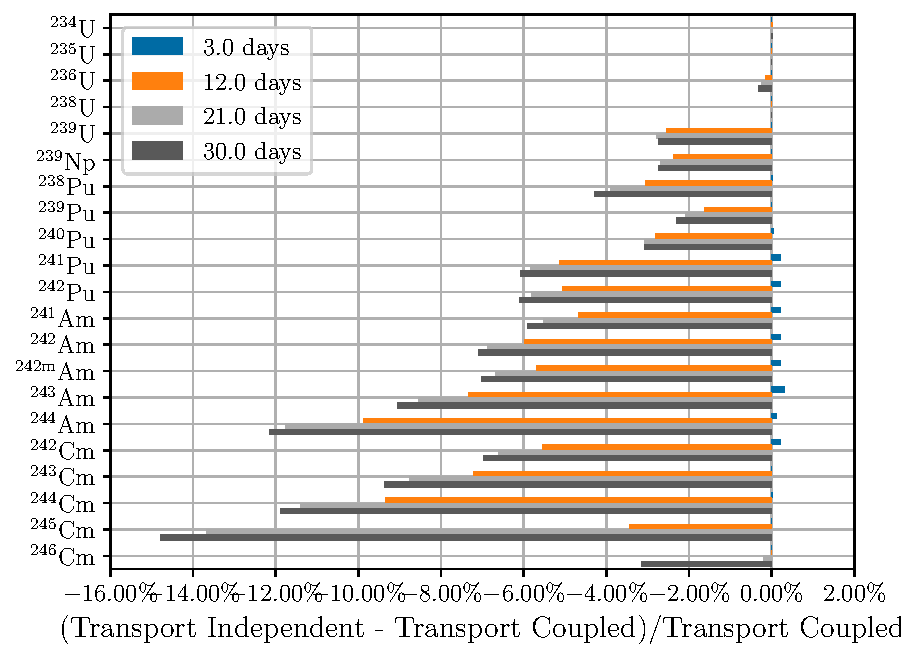
\includegraphics[width=\linewidth]{figs/actinides_casmo8_constant_xs_predictor_fission_q_days.pdf}
        \caption[]{Relative error of predicted actinide concentrations using
        CASMO-8 group structure and 3-day time steps}
        \label{fig:actinides-error-casmo8-xs-days}
    \end{figure}

    \begin{figure}[h!tpb]
        \centering
        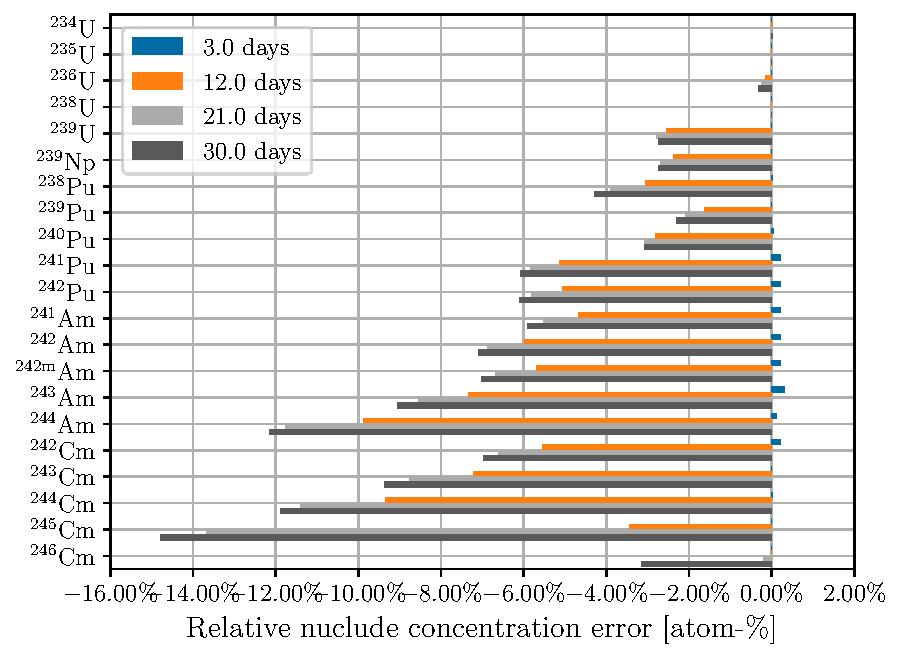
\includegraphics[width=\linewidth]{figs/actinides_casmo40_constant_xs_predictor_fission_q_days.pdf}
        \caption{Relative error of predicted actinide error using
        CASMO-40 group structure and 3-day time steps}
        \label{fig:actinides-error-casmo40-xs-days}
    \end{figure}

    \begin{figure}[h!tpb]
        \centering
        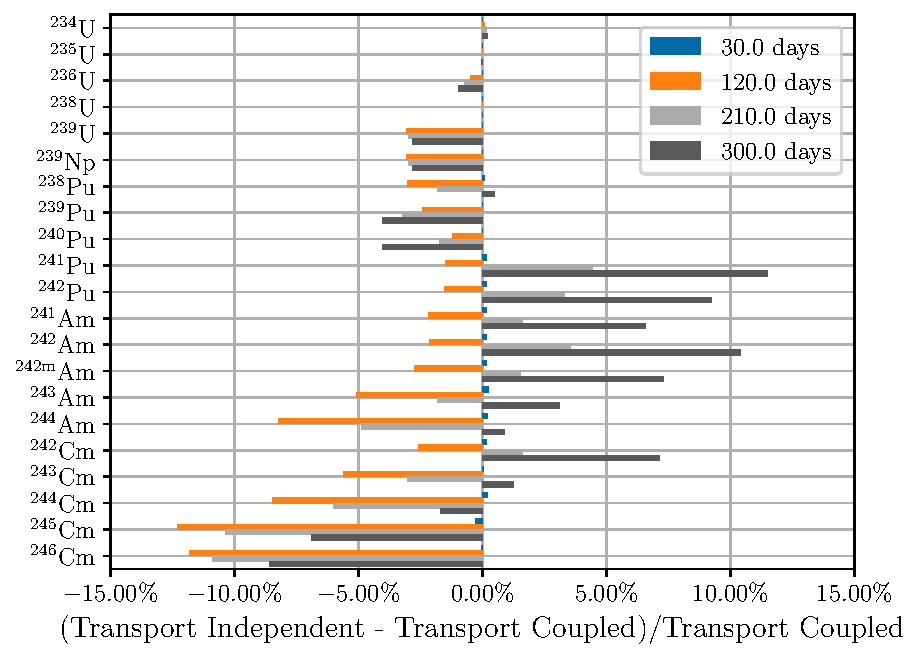
\includegraphics[width=\linewidth]{figs/actinides_casmo8_constant_xs_predictor_fission_q_months.pdf}
        \caption[]{Relative error of predicted actinide concentrations using
        CASMO-8 group structure and 30-day time steps}
        \label{fig:actinides-error-casmo8-xs-months}
    \end{figure}

    \begin{figure}[h!tpb]
        \centering
        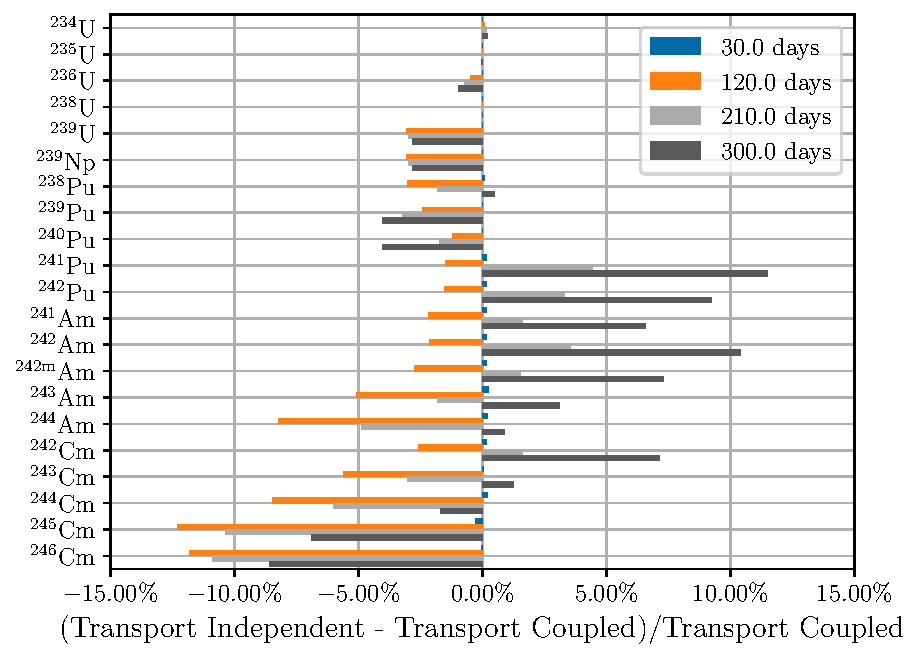
\includegraphics[width=\linewidth]{figs/actinides_casmo40_constant_xs_predictor_fission_q_months.pdf}
        \caption{Relative error of predicted actinide error using
        CASMO-40 group structure and 30-day time steps}
        \label{fig:actinides-error-casmo40-xs-months}
    \end{figure}


    The time savings when using \verb.IndependentOperator. are immense. Whereas
    the transport-coupled simulations each took several hours to complete, the
    transport-independent simulations took seconds to minutes to complete!
